% !TeX root = ../../tfg.tex
% !TeX encoding = utf8
%
%***************************************************************
% Contenido del artículo 3: Avanzamos en la generalización
%***************************************************************

% Teorema 2.2 
\begin{teorema}\label{teo:2_2_denso_función_continua}
    Para cualquier función continua no constate $G$, $r \in \N$ y
    medida de probabilidad $\mu$ o $(\R^r, B^r)$, 
    se tiene que $\pmcg$ es $\dist$-denso en $\fM$. 
\end{teorema} 
\begin{proof}
    Debemos probar que para cualquier función $f \in \fM$ existe una 
    sucesión de funciones $\{h_n\}_{n\in \N}$ contenida en $\pmcg$ y 
    cumpliendo que $\dist(h_n, f) \longrightarrow 0.$

    Consideramos cualquier $f \in \fM$,
    por el lema \ref{lema:A_1_C_es_denso_en_M} sabemos que $\fC$ es $\dist$-denso en $\fM$; 
    es decir, existirá un sucesión $\{f_n\}_{n\in \N}$ de funciones de $\fC$ convergente a 
    $f$.  
    
    Por otra parte sabemos por el teorema \ref{teo:TeoremaConvergenciaRealEnCompactosDefinicionesEsenciales}, 
    que $\pmcg$ es uniformemente denso por compactos en $\fC$, luego en cualquier compacto 
    $K \subset \R^r$ existirá una sucesión (con $n$ fijo) $\{g(n)_m \} _{m \in \N}$ convergente 
    a $f_n$, el término n-ésimo de la sucesión convergente a $g$. 

    Así pues, denotando como $h_n$ al término $g(n)_n$, obtenemos una sucesión de funciones 
    en $\fM$ que converge uniformemente en compactos a $f$ y por el lema \ref{lema:2_2_convergencia_uniforme_en_compactos}
    tenemos que $\dist(h_n, f) \longrightarrow 0$ como queríamos probar.     
\end{proof}

% --- Faltan por demostrar -----
% Lema A.2 
\begin{lema}\label{lema:a_2_paso_previo_denso}
    Sea F una función de activación continua y $\psi$ una \textbf{función de activación} arbitraria. 
    Para cualquier $\epsilon > 0$ existe un elemento $H_{\epsilon}$ de $\sum^1(\psi)$ cumpliendo que
    \begin{equation}
        \sup_{\lambda \in \R} | F(\lambda) - H_{\epsilon}(\lambda) | < \epsilon.
    \end{equation}
\end{lema} 
\begin{proof}
    Procedamos a realizar la siguiente prueba constructiva. 
    Tomamos fijo pero arbitrario un $\epsilon > 0,$ que sin pérdida de generalidad
    supondremos menor que uno 
    \footnote{En caso de ser mayor, se tomará cualquier otro menor que la unidad y la función resultante será igual de válida.}.
    Para que la $H_\epsilon$ pertenezca a $\sum ^1 (\psi)$ deberá de ser de la 
    forma $\sum^{q-1}_{j=1} b_j \psi( A_j(\lambda))$
    debemos encontrar por ende el número de sumatorias, $q-1$; esa misma cantidad de constantes reales $b_j$ y funciones afines $A_j$. 
    

    Para ello tomamos como $q$ a cualquier número natural que cumpla que 
    \begin{equation}\label{eq:lema_a_2_def_q}
        \frac{1}{q} < \frac{\epsilon}{4}.
    \end{equation}

    Fijaremos para cada $j \in \{1,2, ...,q-1\}$ los coeficientes  $b_j$ como $\frac{1}{q}$. 

    Seleccionamos cualquier constante real $M>0$ de tal forma que 
    se cumpla que
    \begin{equation}\label{lema_a_2_psi_m}
        \psi(-M) < \frac{\epsilon}{2q}
        \quad \text{ y } \quad
        \psi(M) > 1 - \frac{\epsilon}{2q}.
    \end{equation} 
    Sabemos que esto es posible ya que por ser $\psi$ una función de activación satisface que 
    $\lim_{\lambda \longrightarrow \infty} \psi(\lambda) = 1$ y que  $\lim_{\lambda \longrightarrow -\infty} \psi(\lambda) = 0$,
    por tanto existirá una constante $M_1$ positiva tal que a partir de ella cualquier
     otra constante $n_1$ mayor o igual que cumpla que 
    $\psi(n_1) > 1 - \frac{\epsilon}{2q}$. También existirá una constante $M_2$ positiva tal que a partir de 
    ella cualquier otra constante $n_2$ mayor o igual tal que que 
    $\psi(-n_2) < \frac{\epsilon}{2q}$. Podemos tomar como $M$ al máximo de $M_1$ y $M_2$.   

    Seleccionaremos ahora los siguientes puntos del dominio
    \begin{equation}\label{lema:2_2_selección_r_F}
        r_j = \sup \left\{ \lambda: F(\lambda) = \frac{j}{q} \right\},
         \text{ con } j \in \{1, ..., q-1\}, 
         \quad \text{ y } \quad
        r_q = \sup \left\{ \lambda: F(\lambda) = 1 - \frac{1}{q} \right\}. 
    \end{equation}
    Que por ser $F$ continua sabemos que existen. 

    Procedemos ahora a definir las distintas aplicaciones afines. 
    Para cualquier reales $s,r$ que cumplan que $r < s$ sea $A_{rs}\in A^1$ la única aplicación afín que satisface que 
    
    \begin{equation}
        A_{rs}(r) = -M \text{ y }  A_{rs}(s) = M. 
    \end{equation} 
    
    Acabamos pues de determinar todos los elements que conforman a $H_\epsilon$, de tal forma que se tiene que
    \begin{equation}
        H_\epsilon(\lambda) = \frac{1}{q} \sum^{q-1}_{j=1} \psi( A_{r_j, r_{j+1}}(\lambda))
    \end{equation}
    y así definida cumple que: 
    \begin{itemize}
        \item Si $\lambda \in (- \infty, r_1]:$
        Se cumple que $\lambda \leq r_1 < r_2 <...< r_q$ luego  
        para todos los $j \in \{1, ..., q-1\}$ las funciones afines satisfacen que 
        $A_{r_j, r_{j+1}}(\lambda) < -M$ y por cómo se fijó la $M$ en la condición \refeq{lema_a_2_psi_m}
        resulta que  $\psi( A_{r_j, r_{j+1}}(\lambda)) < \frac{\epsilon}{2q}$ concluyendo que 
        para $\lambda \in (- \infty, r_1]$
        \begin{equation}
            H_\epsilon(\lambda) = \frac{1}{q} \sum^{q-1}_{j=1} \psi( A_{r_j, r_{j+1}}(\lambda)) 
            <
            \frac{1}{q} \sum^{q-1}_{j=1}  \frac{\epsilon}{2q}
            < 
            \frac{1}{q} (q-1) \frac{\epsilon }{2q}
            <\frac{\epsilon }{2q}
            < \frac{\epsilon }{2}
        \end{equation}
        y por ende, como además $0 \leq F(\lambda) \leq \frac{1}{q} < \frac{\epsilon}{2}$ por cómo se seleccionaron los $r_j$ en 
        \refeq{lema:2_2_selección_r_F} se tiene que 
        \begin{equation}
            | F(\lambda) - H_{\epsilon}(\lambda) | < \frac{\epsilon}{2} + \frac{\epsilon}{2} < \epsilon. 
        \end{equation}

        \item Si $\lambda \in (r_q, +\infty):$
        Se cumple que $r_1 < r_2 <...< r_q <\lambda$ luego  
        para todos los $j \in \{1, ..., q-1\}$ las funciones afines satisfacen que  
        $A_{r_j, r_{j+1}}(\lambda) > M$ y por cómo se fijó la $M$ en \refeq{lema_a_2_psi_m}
        resulta que  $\psi( A_{r_j, r_{j+1}}(\lambda)) > 1-\frac{\epsilon}{2q}$ concluyendo que 
        para $\lambda \in (r_q,+\infty):$
        \begin{equation}
            1 \geq
            H_\epsilon(\lambda) = \frac{1}{q} \sum^{q-1}_{j=1} \psi( A_{r_j, r_{j+1}}(\lambda)) 
            >
                \frac{1}{q} \sum^{q-1}_{j=1}  \left(1-\frac{\epsilon}{2q} \right)
            >
            \frac{(q-1)}{q}  \left(1-\frac{\epsilon}{2q} \right)   
        \end{equation}
        y por ende, como además $\frac{(q-1)}{q}  \left(1-\frac{\epsilon}{2q} \right) <  \frac{q-1}{q} \leq F(\lambda) \leq 1$ por cómo se seleccionaron los $r_j$ en 
        \refeq{lema:2_2_selección_r_F} se tiene que 
        \begin{equation}
            | F(\lambda) - H_{\epsilon}(\lambda) | 
            \leq
            1 - \frac{(q-1)}{q}  \left(1-\frac{\epsilon}{2q} \right)
            = \frac{1}{q} + \frac{\epsilon}{2q}
            < \epsilon.
        \end{equation}
        Donde para acotar $\frac{1}{q}$ hemos usado la desigualdad \refeq{eq:lema_a_2_def_q}.

        \item Si $\lambda \in (r_{j},r_{j+1}]:$
        
        Tenemos por una parte que $\frac{j}{q} < F(\lambda) \leq \frac{j+1}{q}$ y 
        podemos descomponer $H_\epsilon$ en las siguientes sumatorias: 
        \begin{equation}
            \begin{split}
                q H_\epsilon(\lambda) 
                = 
                 \sum^{j-1}_{i=1} \psi( A_{r_i, r_{i+1}}(\lambda))
                + 
                \psi( A_{r_j, r_{j+1}}(\lambda))
                + 
                \sum^{q-1}_{i=j+1} \psi( A_{r_i, r_{i+1}}(\lambda))
            \end{split}
        \end{equation}

        Los términos de la primera sumatoria serán mayores que $\left(1-\frac{\epsilon}{2q} \right)$ y menores o iguales que la unidad, 
        el segundo sumando satisface que 
        $0 \leq q\psi( A_{r_j, r_{j+1}}(\lambda)) \leq 1$
        y para la última sumatoria, todos sus términos serán menores que $\frac{\epsilon}{2q}$ y mayores o iguales que cero.
        De donde resulta que : 
        \begin{equation}
            \frac{j-1}{q}\left(1-\frac{\epsilon}{2q} \right)  
            <
            H_\epsilon(\lambda) 
            <
            \frac{j-1}{q} 
            + 
            \frac{1}{q} 
            + 
            \frac{q-j}{q} \frac{\epsilon}{2q} 
        \end{equation}
        Concluyendo que 
        \begin{equation}
            F(\lambda), H_\epsilon(\lambda) 
            \in 
            \left[
                \frac{j-1}{q}\left(1-\frac{\epsilon}{2q}\right),
                \frac{j+1}{q}
            \right]
        \end{equation}
        y por tanto: 
        \begin{equation}
            | F(\lambda) - H_{\epsilon}(\lambda) | 
            \leq \frac{j+1}{q} -  \frac{j-1}{q}\left(1-\frac{\epsilon}{2q}\right)
            = 
            \frac{2}{q} + \frac{j-1}{q}\frac{\epsilon}{2q}
            < \frac{\epsilon}{2} + \frac{\epsilon}{2}
            < \epsilon.
        \end{equation}
        Donde para acotar $\frac{2}{q}$ hemos usado la desigualdad \refeq{eq:lema_a_2_def_q}.
    \end{itemize}
    La acotación $| F(\lambda) - H_{\epsilon}(\lambda) | < \epsilon$ se cumple para todo
    \begin{equation}
        \lambda \in (- \infty, r_1] \cup (r_q,+\infty) \cup_{j \in \{1, ..., q-1\}} (r_{j},r_{j+1}] = \R,
    \end{equation}
    probando con ello lo buscado.
\end{proof}      

% Teorema 2.3
\begin{teorema}
    Para cualquier función de activación $\psi$, $r$ natural positivo y
    medida de probabilidad $\mu$ en $(\R^r, B^r)$, 
    se tiene que $\rrnng$ es uniformemente denso en compactos
    en $\fC$ y denso en $\fM$ de acorde a la distancia $\dist$. 
\end{teorema}
\begin{proof}
    En virtud del lema \ref{lema:2_2_convergencia_uniforme_en_compactos} y del 
    teorema \ref{teo:2_2_denso_función_continua} basta con probar que 
    $\rrnng$ es uniformemente denso en compactos de $\sum \prod^r(F)$, 
    donde $F$ es una función de activación continua 
    \footnote{el razonamiento 
    por el que con esta hipótesis es suficiente es idéntico al realizado para la 
    demostración del teorema \ref{teo:2_2_denso_función_continua}.}.

    Para ello basta ver que cualquier función de la forma $\prod_{k=1}^l F(A_k(\cdot))$
    puede ser uniformemente aproximada por una una sucesión de funciones de $\rrnng$.

    Fijamos un $\epsilon > 0$  de manera arbitraria. 
    Gracias a la continuidad de la norma y de la operación multiplicación, existirá un $\delta >0$
    tal que para cualesquiera números reales $0 \leq a_k, b_k \leq 1,$ con $k \in \{1,...,l\}$ 
    se satisfagan que $|a_k -b_k| < \delta$ se cumple que 
    \begin{equation} \label{eq:teorema_2_3__1}
        \left| 
            \prod^l_{k=1} a_k - \prod^l_{k=1} b_k 
        \right| 
        < 
        \epsilon.
    \end{equation}

    Por el lema \ref{lema:a_2_paso_previo_denso} existe una función 
    $H_{\delta}(\cdot) = \sum_{t=1}^T \beta_t \psi(A_t(\cdot))$
    cumpliendo que 

    \begin{equation}
        \sup_{\lambda \in \R} |F(\lambda) - H_{\delta}(\lambda) | < \delta.
    \end{equation}

    Se satisface con la cota suficiente de la desigualdad \refeq{eq:teorema_2_3__1} por lo que 
    resulta 
    \begin{equation}\label{eq:teorema2_3__3}
        \sup_{x \in \R^r} 
        \left| 
            \prod ^l_{k=1} F(A_k(x))
            -
            \prod ^l_{k=1} H_\delta(A_k(x))
        \right| 
        < 
        \epsilon.
    \end{equation} 
    
    Puesto que $H_\delta$ es de la forma  $\sum_{t=1}^T \beta_t \psi(A^1_t(\cdot))$ 
    y porque $A^1_t(A_k(\cdot)) \in A^r$ se tiene por la desigualdad \ref{eq:teorema2_3__3} que 
    $\prod ^l_{k=1} H_\delta(A_k(\cdot)) \in \rrnng.$

    Por lo tanto c $\prod ^l_{k=1} F(A_k(\cdot))$ puede ser 
    aproximado por elementos de $\rrnng$ y acabamos de probar con ello lo buscado. 
\end{proof} 

%% Faltan  por probar 
%Lema A.3
\begin{lema}\label{lema:A_3_función_activación_continua_con_arbitaria}
    Para cada función de activación $\psi$, cada $\epsilon >0$
    y cada $M>0$ existe una función 
    $cos_{M,\epsilon} \in \sum^1(\psi)$ tal que 
    \begin{equation}
        \sup_{ \lambda \in [-M, +M]}
        |\cos_{M,\epsilon}(\lambda) - \cos(\lambda)|
        < 
        \epsilon. 
    \end{equation}
\end{lema}
\begin{proof}
    Sea $F$ la función de activación \textit{cosine squasher} de Gallant and White (1988) definida 
    en \ref{def:funcion_activacion_articulo}

    Comenzaremos probando que para un intervalo acotado $[-M, M]$, existe $H \in \sum(F)$ 
    tal que para todo elemento $\lambda \in [-M, M]$ se cumpla que 

    \begin{equation}
        H(\lambda) = \cos(\lambda).
    \end{equation}

    Calcularemos $H \in \sum(F)$  de forma constructiva: 
    \begin{equation}
        F(\lambda )= \left(1 + \cos\left(\lambda -\frac{\pi}{2} \right) \frac{1}{2}\right) 
         1_{\{\frac{-\pi}{2} \leq \lambda \leq  \frac{\pi}{2}\}}
         +
         1_{\{ \frac{\pi}{2} < \lambda \}}.
    \end{equation}
    
    \begin{figure}[h]
        \centering
        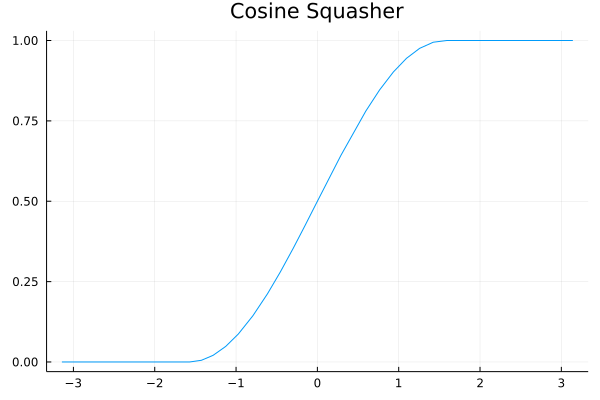
\includegraphics[width=.7\textwidth]{articulo_rrnn_aproximadores_universales/cosineSquasher.png}
        \caption{Función \textit{cosine squasher}}
        \label{fig:cosine_squaser}
    \end{figure}

    Se tiene pues que para cualquier $\lambda \in \left[ \frac{-\pi}{2}, \frac{\pi}{2}\right]$

    \begin{equation}
        2 F(\lambda)-1 = \cos \left( \lambda - \frac{\pi}{2}\right)
    \end{equation}

    Que haciendo $\mu = \lambda - \frac{\pi}{2}$ resulta que para cualquier
    $\mu \in [-\pi, 0]$
    \begin{equation}
        \cos(\mu) = 2 F \left(\mu + \frac{\pi}{2} \right)  -1 
    \end{equation}

    Además, puesto que $F(\mu + 2 \pi M) = 1$ para todo $\mu \in [-M, M] \supset [-\pi, 0]$ tenemos que
    para cualquier $\mu \in [-\pi, 0]$
    \begin{equation}
        \cos(\mu) = 2 F \left(\mu + \frac{\pi}{2} \right)  - F(\mu + 2 \pi M) 
    \end{equation}

    \begin{figure}[h]
        \centering
        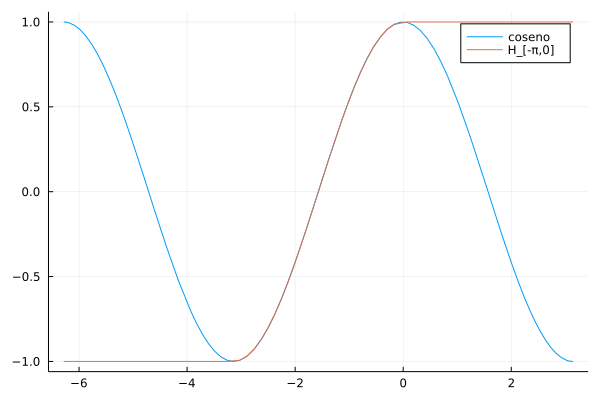
\includegraphics[width=.7\textwidth]{articulo_rrnn_aproximadores_universales/H_menos_pi_0.png}
        \caption{Comparativa $H_{[-\pi, 0]}$ con la función coseno real. }
        \label{fig:coseno_vs_H_menos_pi_cero}
    \end{figure}

    De manera generalizada denotaremos como $H_{[M_1,M_2 ]}$ a la función 
     existe $H_{[M_1,M_2 ]} \in \sum(F)$ 
    tal que para todo elemento $\lambda \in [M_1, M_2]$ se cumpla que 
    \begin{equation}
        H_{[M_1,M_2 ]}(\lambda) = \cos(\lambda)
    \end{equation}

    Por tanto $H_{[-\pi, 0]}$ viene definida como  
    \begin{equation}
        H_{[-\pi, 0]} = 2 F \left(\mu + \frac{\pi}{2} \right)  - F(\mu + 2 \pi M) 
    \end{equation}

    Por la simetría de la función coseno resulta que 
    para todo $\mu \in [0, \pi]$
    \begin{equation}
        \cos(\mu) = \cos(-\mu) = H_{[-\pi, 0]}(-\mu)
    \end{equation}
    \begin{figure}[h]
        \centering
        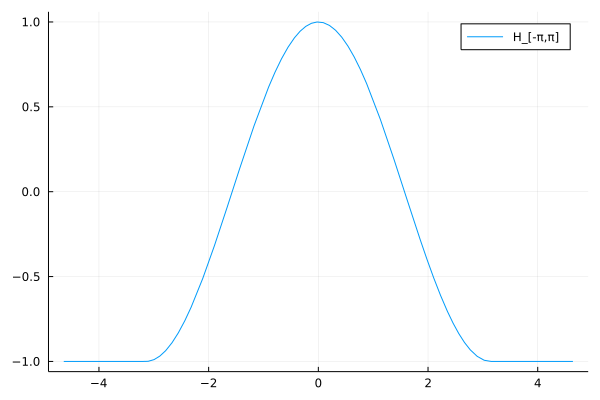
\includegraphics[width=.7\textwidth]{articulo_rrnn_aproximadores_universales/H_menos_pi_mas_pi.png}
        \caption{Función $H_{[-\pi, \pi]}$. }
        \label{fig:H_menos_pi_mas_pi}
    \end{figure}

    Así pues podemos definir 
    \begin{equation}
        \begin{split}
            H_{[-\pi, \pi ]}(\mu) &= H_{[-\pi, 0]}(\mu) + H_{[-\pi, 0]}(-\mu) - 1 \\
            &= H_{[-\pi, 0]}(\mu) + H_{[-\pi, 0]}(-\mu) - F(\mu + 2 \pi M). 
        \end{split} 
    \end{equation}  

    Por ser el coseno una función periódica es fácil ver que 
    considerando un natural $N$ que satisfaga que $2 \pi N \geq M$
  
    \begin{equation}
    \begin{split}
        H_{[-2\pi N, 2 \pi N]} (\lambda) = 
        \sum_{i=1}^N (H_{[-\pi, \pi ]}(\lambda + 2 \pi i) +1) 
        + H_{[-\pi, \pi ]}(\lambda)  \\
        - \sum_{i=1}^N (H_{[-\pi, \pi ]}(- \lambda + 2 \pi i - \pi) +1),
    \end{split}
\end{equation}
\begin{equation}
    \begin{split}
        H_{[-2\pi N, 2 \pi N]} (\lambda) 
        =  H_{[-\pi, \pi ]}(\lambda) + 
        \sum_{i=1}^N (
            H_{[-\pi, \pi ]}(\lambda + 2 \pi i)
            - 
            H_{[-\pi, \pi ]}(- \lambda + 2 \pi i - \pi)
        ) .         
    \end{split}
    \end{equation}

      % Ejemplos de la función H final
      \begin{figure}[h]
        \centering
        \begin{subfigure}[b]{0.45\textwidth}
            \centering
            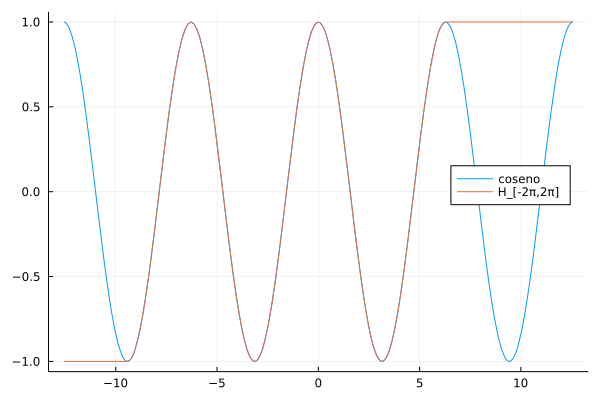
\includegraphics[width=\textwidth]{articulo_rrnn_aproximadores_universales/H_[-2π,2π].png}
            \caption{Función $H_{[-2\pi, 2\pi]}$ con $N=1$.}
            \label{fig:H_con_M}
        \end{subfigure}
        \hfill
        \begin{subfigure}[b]{0.45\textwidth}
            \centering
            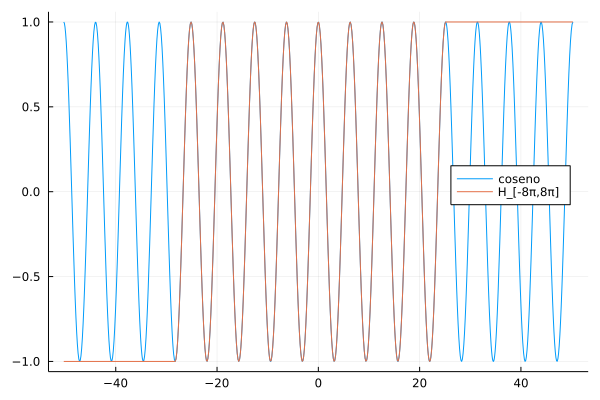
\includegraphics[width=\textwidth]{articulo_rrnn_aproximadores_universales/H_[-8π,8π].png}
            \caption{Función $H_{[-8\pi, 8\pi]}$ con $N=4$. }
        \end{subfigure}
        \hfill
        \caption{Ejemplos de funciones $H_{[-M, M]}$}
    \end{figure}

    Está claro que por ser $2 \pi N \geq M$ la función $H_{[-M, M]}$ será la restricción de la anterior, es decir: 

    \begin{equation}
        H_{[-M, M]} = H_{[-2\pi N, 2 \pi N]_{|[-M, M]}}.
    \end{equation}

    
    Así definida $H_{[-2\pi N, 2 \pi N]}$
    pertenecerá a $\sum(F)$ o lo que es de nuestro interés, estará 
    formada por una combinación finita, supongamos que $K$, 
    sumas y restas finita de $F \circ A_i$ con $A_i$ una función afín. 
    Por ser $F$ una función de activación continua gracias al
    lema \ref{lema:a_2_paso_previo_denso}, 
    existirá $W_{ \frac{\epsilon}{k}} \in \sum(\psi)$ tal que 
    podremos acotar $|F - W_{ \frac{\epsilon}{k}} | < \frac{\epsilon}{k}$ en todo $\R$.

    Además, como las transformaciones afines $A_i$ solo son traslaciones,
    para cada $i \in \{1,..K\}$ se cumple que 
     $W_{ \frac{\epsilon}{k}} \circ A_i \in \sum(\psi)$ y se mantiene que 
    \begin{equation}
        |F \circ A_i - W_{ \frac{\epsilon}{k}} \circ A_i | < \frac{\epsilon}{k}. 
    \end{equation}


    Recopilemos pues, tenemos que para $2\pi N \geq M$ y en el dominio $\lambda \in [-M, M]$: 
    \begin{equation}
        H_{[-M, M]} (\lambda) = 
        H_{[-2\pi N, 2 \pi N]}(\lambda) = 
        \sum_{i=1}^k \alpha_i F( A_i(\lambda)) \quad \alpha_i \in \{-1,1\}.
    \end{equation}
    fijando tales $\alpha_i \in \{-1,1\}$ y las traslaciones $A_i$ definimos 
    \begin{equation}
        \cos_{M, \epsilon}(\lambda) = \sum_{i=1}^k 
        \alpha_i  W_{ \frac{\epsilon}{k}}(A_i(\lambda)). 
    \end{equation}

    De esta manera, para cualquier $\lambda \in [-M, M]$

    \begin{equation}
        \begin{split}
            |\cos_{M,\epsilon}(\lambda) - \cos(\lambda)| 
            &= |\cos_{M,\epsilon}(\lambda) - \cos(\lambda) \pm  H_{[- M, M]}(\lambda)| \\
            &\leq
            |\cos(\lambda) -  H_{[- M, M]}(\lambda)|
            + 
            | \cos_{M,\epsilon}(\lambda) -  H_{[- M, M]}(\lambda)|  \\
            &\leq  0 
            + | \cos_{M,\epsilon}(\lambda) -  H_{[- M, M]}(\lambda)| \\
            & \leq  \sum_{i=1}^k 
            |  W_{ \frac{\epsilon}{k}}(A_i(\lambda)) 
            -
            F( A_i(\lambda))
             | \\
             & <   \sum_{i=1}^k \frac{\epsilon}{k} = \epsilon .
        \end{split}
    \end{equation}

    Dando con esto por concluida la demostración. 
 
\end{proof}

%Lema 4.A
\begin{lema}\label{lema:A_4_sum_cos_aproxima}
    Sea $g(\cdot) = \sum_{j=1}^q \beta_j \cos(A_j(\cdot))$ con 
    $A_j \in A^r$.
    Para cualquier función de activación $\psi$, 
    cualquier compacto $K \subset \R^r$
    y cualquier $\epsilon > 0$
    existe $f \in \sum^r(\psi)$ para el cual se cumple que 
    \begin{equation}
        \sup_{x \in K} 
        |g(x) - f(x)| < \epsilon.
    \end{equation}
\end{lema}
\begin{proof}
    Puesto que $K$ es un compacto, el número de sumatorias $q$
    es finito y $A_j$ son funciones continuas
    , existe
     $M$ un número real positivo  cumpliendo que
    \begin{equation}
        A_i(K) \subseteq [-M, M] 
        \quad 
        \text{para todo } j \in \{1, ..., q \}. 
    \end{equation} 

    También existe un real $B$, que es el máximo de las normas 
    los coeficientes de $g$. 
    \begin{equation}
        B = \sup \{ |\beta_j| :  j \in \{1, ..., q \}\}
    \end{equation}

    En virtud del lema \ref{lema:A_3_función_activación_continua_con_arbitaria}
    podemos encontrar un 
    $\cos_{M, \frac{\epsilon}{q B}} \in \sum(\psi)$ cumpliendo que
    \begin{equation}
        \sup_{\lambda \in [-M, M]} | 
        \cos_{M, \frac{\epsilon}{q B}}(\lambda)
        - 
        cos(\lambda)
        | 
        < \frac{\epsilon}{q B} 
    \end{equation}
    por lo que para cualquier  $j \in \{1, ..., q \}\}$   se tiene que 
    \begin{equation}
        \sup_{x \in K} | 
        \cos_{M, \frac{\epsilon}{q B}}(A_j(x))
        - 
        cos(A_j(x))
        | 
        \leq  
        \sup_{\lambda \in [-M, M]} | 
        \cos_{M, \frac{\epsilon}{q B}}(\lambda)
        - 
        cos(\lambda)
        | 
        < \frac{\epsilon}{q B}. 
    \end{equation}

    Definamos ahora $f$ como 
    \begin{equation}
        f(x) = \sum_{j=1}^q \beta_j \cos_{M, \frac{\epsilon}{q B}}(A_j(x)).
    \end{equation}
    Puesto que $\cos_{M, \frac{\epsilon}{q B}} \in \sum(\psi)$ entonces 
    $f \in \sum^r(\psi)$ y satisface además que 

    \begin{equation}
        \begin{split}
        \sup_{x \in K} | f(x) - g(x)| 
        \leq
        \sup_{\lambda \in [-M, M]} 
        | \sum_{j=1}^q \beta_j \cos_{M, \frac{\epsilon}{q B}}(\lambda )
         - 
         \sum_{j=1}^q \beta_j \cos(\lambda )|  \\
        \leq
        \sup_{\lambda \in [-M, M]} 
        \sum_{j=1}^q 
            |\beta_j|
            |
                \cos_{M, \frac{\epsilon}{q B}}(\lambda)
                -
                \cos(\lambda)
            |   
            <
            \sup_{\lambda \in [-M, M]} 
            \sum_{j=1}^q   
                B
                \frac{\epsilon}{q B}
            = \epsilon.
        \end{split}
    \end{equation}
     Con lo que acabamos de probar la tesis del lema. 
\end{proof}


%Lema A.5 
\begin{lema} \label{lema:A_5_uniformemente_denso_compactos}
    Para cualquier función de activación $\psi$ se tiene que 
    $\rrnn$ es uniformemente denso en compactos de $\fC.$
\end{lema}
\begin{proof}
    En virtud del lema \ref{lema:A_4_sum_cos_aproxima} 
    bastaría probar que $\sum^r(cos)$ es uniformemente 
    denso en compactos, ya que hemos visto que $\rrnn$ 
    es denso en $\sum^r(cos)$. 

    Veamos ahora que $\sum^r(cos) = \sum \prod^r(cos)$ 
    donde recordamos que $\sum \prod^r(cos)$ se correspondía
    con el espacio de los polinomios trigonométricos. 
    \begin{equation}
        \sum \prod^r(\cos) = 
        \left\{
            \sum_{j=1}^q \beta_j 
            \prod_{k=1}^{l_j} \cos(A_{j,k}(\cdot)) 
            : q, l_j \in \N, \beta_j \in \R, A_{j,k}\in A^r
        \right\}
    \end{equation}
    Y  $\sum^r(cos)$ el caso particular de los polinomios anteriores 
    de grado uno. 
    
    Luego está claro que $\sum^r(cos) \subseteq \sum \prod^r(cos).$
    Traigamos a colación las siguientes igualdades trigonométricas:

    Para cualesquiera números reales $A,B$ 
    \begin{equation}
        \begin{split}
            &\cos(A + B)  = 
            \cos(A)\cos(B) - \sin(A)\sin(B) \\
            &\cos(A - B)  = 
            \cos(A)\cos(B) + \sin(A)\sin(B).
        \end{split}
    \end{equation}

    Por lo que sumando
    \begin{equation}
        \begin{split}
            \cos(A + B)  + \cos(A - B)
            = 2\cos(A)\cos(B).
        \end{split} 
    \end{equation}  
    y de manera general si definimos 
    \begin{equation}
        \Lambda_l = \{
            (x_1, x_2, ..., x_l) : 
            x_1 = 1, x_i \in \{-1, 1\} 
            \text{ para cualquier } 1 < i \leq l
        \}
    \end{equation}

    \begin{equation}
        \prod^l_{k=1} cos(A_k) = 
        \frac{1}{2^{l-1}}(\sum_{x \in \Lambda_l}
         \cos(\sum_{i=1}^l x_i A_i)). 
    \end{equation}

    Por lo que cada elemento 
    $\sum_{j=1}^q \beta_j \prod_{k=1}^{l_j} \cos(A_{j,k}(\cdot)) \in \sum \prod^r(cos)$
    podrá ser expresado como 
    $\sum_{j=1}^q \beta_j \prod_{k=1}^{l_j} \cos(A_{j,k}(\cdot)) = 
    \sum_{j=1}^t \alpha_j \cos(A_{j,k}(\cdot))$, es decir, como un elemento 
    de $\sum^r(cos)$. Concluimos como queríamos que son iguales
    los espacios
    $\sum^r(cos)$ y $\sum \prod^r(cos)$. 

    Finalmente gracias al teorema \ref{teo:TeoremaConvergenciaRealEnCompactosDefinicionesEsenciales}
    por ser  el $\cos$ una función real continua no constante sabemos que 
    $\sum \prod^r(\cos)$ es uniformemente denso en compactos en $\fC$ 
    probando con esto el resultado buscado. 
    
\end{proof}

Estamos ya en condiciones de probar el resultado clave del artículo. 

% Teorema 2.4
\begin{teorema} \label{teo:2_4_rrnn_densas_M}
    Para cualquier función de activación $\psi$, $r \in \N$ y
    medida de probabilidad $\mu$ o $(\R^r, B^r)$, 
    se tiene que $\rrnn$ es uniformemente denso en compactos
    en $\fC$ y denso en $\fM$ de acorde a la distancia $\dist$. 
\end{teorema}
\begin{proof}
Por el lema anterior \ref{lema:A_5_uniformemente_denso_compactos}
acabamos de ver que $\rrnn$ es uniformemente denso en compactos de $\fC$
y gracias al lema \ref{lema:2_2_convergencia_uniforme_en_compactos} 
(Si $\{f_n\}$ es una sucesión de funciones en $\fM$ que converge
uniformemente en un compacto a $f$ entonces $\rho_{\mu}(f_n, f) \longrightarrow 0$.)
esto implica 
que $\rrnn$ sea $\dist$-denso en $\fC$. 

Finalmente como consecuencia del 
lema \ref{lema:A_1_C_es_denso_en_M}  que indica que 
para cualquier medida finita $\mu$ se tiene que $\fC$ es denso en 
$\fM$ para la distancia $\rho_\mu$
se tiene por la transitividad de ser denso (ver mismo razonamiento que el 
usado para la demostración del teorema \ref{teo:2_2_denso_función_continua})
$\rrnn$ es $\dist$-denso en $\fM$.
\end{proof}

\subsubsection{Relevancia del teorema de aproximación de funciones medibles \ref{teo:2_4_rrnn_densas_M}}

Notemos que  $\rrnn$ representa el conjunto de 
las redes neuronales \textit{feedforward} con tan solo una capa oculta, luego 
acabamos de probar que las redes neuronales \textit{feedforward} con 
tan solo una capa oculta son capaces de aproximar \textit{con un error uniformemente} 
cualquier función continua y aproximar \textit{a secas} cualquier
función medible 
con cualquier medida $\mu$, distancia $\dist$, independiente de la 
función de activación $\mu$ seleccionada (ya sea continua o no) 
y con cualquier dimensión $r$ del espacio de entrada. 

 
